\documentclass[twoside]{book}

% Packages required by doxygen
\usepackage{fixltx2e}
\usepackage{calc}
\usepackage{doxygen}
\usepackage[export]{adjustbox} % also loads graphicx
\usepackage{graphicx}
\usepackage[utf8]{inputenc}
\usepackage{makeidx}
\usepackage{multicol}
\usepackage{multirow}
\PassOptionsToPackage{warn}{textcomp}
\usepackage{textcomp}
\usepackage[nointegrals]{wasysym}
\usepackage[table]{xcolor}

% Font selection
\usepackage[T1]{fontenc}
\usepackage[scaled=.90]{helvet}
\usepackage{courier}
\usepackage{amssymb}
\usepackage{sectsty}
\renewcommand{\familydefault}{\sfdefault}
\allsectionsfont{%
  \fontseries{bc}\selectfont%
  \color{darkgray}%
}
\renewcommand{\DoxyLabelFont}{%
  \fontseries{bc}\selectfont%
  \color{darkgray}%
}
\newcommand{\+}{\discretionary{\mbox{\scriptsize$\hookleftarrow$}}{}{}}

% Page & text layout
\usepackage{geometry}
\geometry{%
  a4paper,%
  top=2.5cm,%
  bottom=2.5cm,%
  left=2.5cm,%
  right=2.5cm%
}
\tolerance=750
\hfuzz=15pt
\hbadness=750
\setlength{\emergencystretch}{15pt}
\setlength{\parindent}{0cm}
\setlength{\parskip}{3ex plus 2ex minus 2ex}
\makeatletter
\renewcommand{\paragraph}{%
  \@startsection{paragraph}{4}{0ex}{-1.0ex}{1.0ex}{%
    \normalfont\normalsize\bfseries\SS@parafont%
  }%
}
\renewcommand{\subparagraph}{%
  \@startsection{subparagraph}{5}{0ex}{-1.0ex}{1.0ex}{%
    \normalfont\normalsize\bfseries\SS@subparafont%
  }%
}
\makeatother

% Headers & footers
\usepackage{fancyhdr}
\pagestyle{fancyplain}
\fancyhead[LE]{\fancyplain{}{\bfseries\thepage}}
\fancyhead[CE]{\fancyplain{}{}}
\fancyhead[RE]{\fancyplain{}{\bfseries\leftmark}}
\fancyhead[LO]{\fancyplain{}{\bfseries\rightmark}}
\fancyhead[CO]{\fancyplain{}{}}
\fancyhead[RO]{\fancyplain{}{\bfseries\thepage}}
\fancyfoot[LE]{\fancyplain{}{}}
\fancyfoot[CE]{\fancyplain{}{}}
\fancyfoot[RE]{\fancyplain{}{\bfseries\scriptsize Generated by Doxygen }}
\fancyfoot[LO]{\fancyplain{}{\bfseries\scriptsize Generated by Doxygen }}
\fancyfoot[CO]{\fancyplain{}{}}
\fancyfoot[RO]{\fancyplain{}{}}
\renewcommand{\footrulewidth}{0.4pt}
\renewcommand{\chaptermark}[1]{%
  \markboth{#1}{}%
}
\renewcommand{\sectionmark}[1]{%
  \markright{\thesection\ #1}%
}

% Indices & bibliography
\usepackage{natbib}
\usepackage[titles]{tocloft}
\setcounter{tocdepth}{3}
\setcounter{secnumdepth}{5}
\makeindex

% Hyperlinks (required, but should be loaded last)
\usepackage{ifpdf}
\ifpdf
  \usepackage[pdftex,pagebackref=true]{hyperref}
\else
  \usepackage[ps2pdf,pagebackref=true]{hyperref}
\fi
\hypersetup{%
  colorlinks=true,%
  linkcolor=blue,%
  citecolor=blue,%
  unicode%
}

% Custom commands
\newcommand{\clearemptydoublepage}{%
  \newpage{\pagestyle{empty}\cleardoublepage}%
}

\usepackage{caption}
\captionsetup{labelsep=space,justification=centering,font={bf},singlelinecheck=off,skip=4pt,position=top}

%===== C O N T E N T S =====

\begin{document}

% Titlepage & ToC
\hypersetup{pageanchor=false,
             bookmarksnumbered=true,
             pdfencoding=unicode
            }
\pagenumbering{alph}
\begin{titlepage}
\vspace*{7cm}
\begin{center}%
{\Large My Project }\\
\vspace*{1cm}
{\large Generated by Doxygen 1.8.13}\\
\end{center}
\end{titlepage}
\clearemptydoublepage
\pagenumbering{roman}
\tableofcontents
\clearemptydoublepage
\pagenumbering{arabic}
\hypersetup{pageanchor=true}

%--- Begin generated contents ---
\chapter{Hierarchical Index}
\section{Class Hierarchy}
This inheritance list is sorted roughly, but not completely, alphabetically\+:\begin{DoxyCompactList}
\item \contentsline{section}{csis3700\+:\+:collision}{\pageref{classcsis3700_1_1collision}}{}
\item \contentsline{section}{csis3700\+:\+:image\+\_\+library}{\pageref{classcsis3700_1_1image__library}}{}
\item \contentsline{section}{csis3700\+:\+:image\+\_\+sequence}{\pageref{classcsis3700_1_1image__sequence}}{}
\item \contentsline{section}{csis3700\+:\+:image\+\_\+with\+\_\+offset}{\pageref{classcsis3700_1_1image__with__offset}}{}
\item \contentsline{section}{csis3700\+:\+:keyboard\+\_\+manager}{\pageref{classcsis3700_1_1keyboard__manager}}{}
\item \contentsline{section}{csis3700\+:\+:rectangle}{\pageref{classcsis3700_1_1rectangle}}{}
\item \contentsline{section}{csis3700\+:\+:sprite}{\pageref{classcsis3700_1_1sprite}}{}
\begin{DoxyCompactList}
\item \contentsline{section}{csis3700\+:\+:obstruction\+\_\+sprite}{\pageref{classcsis3700_1_1obstruction__sprite}}{}
\item \contentsline{section}{csis3700\+:\+:phys\+\_\+sprite}{\pageref{classcsis3700_1_1phys__sprite}}{}
\begin{DoxyCompactList}
\item \contentsline{section}{csis3700\+:\+:player\+\_\+sprite}{\pageref{classcsis3700_1_1player__sprite}}{}
\end{DoxyCompactList}
\end{DoxyCompactList}
\item \contentsline{section}{csis3700\+:\+:vec2d}{\pageref{classcsis3700_1_1vec2d}}{}
\item \contentsline{section}{csis3700\+:\+:world}{\pageref{classcsis3700_1_1world}}{}
\end{DoxyCompactList}

\chapter{Class Index}
\section{Class List}
Here are the classes, structs, unions and interfaces with brief descriptions\+:\begin{DoxyCompactList}
\item\contentsline{section}{\hyperlink{classcsis3700_1_1collision}{csis3700\+::collision} }{\pageref{classcsis3700_1_1collision}}{}
\item\contentsline{section}{\hyperlink{classcsis3700_1_1image__library}{csis3700\+::image\+\_\+library} }{\pageref{classcsis3700_1_1image__library}}{}
\item\contentsline{section}{\hyperlink{classcsis3700_1_1image__sequence}{csis3700\+::image\+\_\+sequence} }{\pageref{classcsis3700_1_1image__sequence}}{}
\item\contentsline{section}{\hyperlink{classcsis3700_1_1image__with__offset}{csis3700\+::image\+\_\+with\+\_\+offset} }{\pageref{classcsis3700_1_1image__with__offset}}{}
\item\contentsline{section}{\hyperlink{classcsis3700_1_1keyboard__manager}{csis3700\+::keyboard\+\_\+manager} }{\pageref{classcsis3700_1_1keyboard__manager}}{}
\item\contentsline{section}{\hyperlink{classcsis3700_1_1obstruction__sprite}{csis3700\+::obstruction\+\_\+sprite} }{\pageref{classcsis3700_1_1obstruction__sprite}}{}
\item\contentsline{section}{\hyperlink{classcsis3700_1_1phys__sprite}{csis3700\+::phys\+\_\+sprite} }{\pageref{classcsis3700_1_1phys__sprite}}{}
\item\contentsline{section}{\hyperlink{classcsis3700_1_1player__sprite}{csis3700\+::player\+\_\+sprite} }{\pageref{classcsis3700_1_1player__sprite}}{}
\item\contentsline{section}{\hyperlink{classcsis3700_1_1rectangle}{csis3700\+::rectangle} }{\pageref{classcsis3700_1_1rectangle}}{}
\item\contentsline{section}{\hyperlink{classcsis3700_1_1sprite}{csis3700\+::sprite} }{\pageref{classcsis3700_1_1sprite}}{}
\item\contentsline{section}{\hyperlink{classcsis3700_1_1vec2d}{csis3700\+::vec2d} }{\pageref{classcsis3700_1_1vec2d}}{}
\item\contentsline{section}{\hyperlink{classcsis3700_1_1world}{csis3700\+::world} }{\pageref{classcsis3700_1_1world}}{}
\end{DoxyCompactList}

\chapter{Class Documentation}
\hypertarget{classcsis3700_1_1collision}{}\section{csis3700\+:\+:collision Class Reference}
\label{classcsis3700_1_1collision}\index{csis3700\+::collision@{csis3700\+::collision}}
\subsection*{Public Member Functions}
\begin{DoxyCompactItemize}
\item 
\mbox{\Hypertarget{classcsis3700_1_1collision_a28ce4cf4d73a43840adaf882a7f680da}\label{classcsis3700_1_1collision_a28ce4cf4d73a43840adaf882a7f680da}} 
{\bfseries collision} (\hyperlink{classcsis3700_1_1sprite}{sprite} $\ast$p1, \hyperlink{classcsis3700_1_1sprite}{sprite} $\ast$p2)
\item 
\mbox{\Hypertarget{classcsis3700_1_1collision_a5a0054399a8f03e0ad9b10c70ced45c0}\label{classcsis3700_1_1collision_a5a0054399a8f03e0ad9b10c70ced45c0}} 
void {\bfseries resolve} ()
\item 
\mbox{\Hypertarget{classcsis3700_1_1collision_a317f770f60f10889e7e3d9c54544dd56}\label{classcsis3700_1_1collision_a317f770f60f10889e7e3d9c54544dd56}} 
bool {\bfseries is\+\_\+active} () const
\item 
\mbox{\Hypertarget{classcsis3700_1_1collision_a52ebb041711cf7b802715bf12270e8ab}\label{classcsis3700_1_1collision_a52ebb041711cf7b802715bf12270e8ab}} 
\hyperlink{classcsis3700_1_1rectangle}{rectangle} {\bfseries collision\+\_\+rectangle} () const
\item 
\mbox{\Hypertarget{classcsis3700_1_1collision_a718673acc32ae44dda81f4a931037be3}\label{classcsis3700_1_1collision_a718673acc32ae44dda81f4a931037be3}} 
bool {\bfseries operator$<$} (const \hyperlink{classcsis3700_1_1collision}{collision} \&other) const
\end{DoxyCompactItemize}


The documentation for this class was generated from the following files\+:\begin{DoxyCompactItemize}
\item 
collision.\+h\item 
collision.\+cpp\end{DoxyCompactItemize}

\hypertarget{classcsis3700_1_1image__library}{}\section{csis3700\+:\+:image\+\_\+library Class Reference}
\label{classcsis3700_1_1image__library}\index{csis3700\+::image\+\_\+library@{csis3700\+::image\+\_\+library}}
\subsection*{Public Member Functions}
\begin{DoxyCompactItemize}
\item 
\mbox{\Hypertarget{classcsis3700_1_1image__library_adea94b7de53bcbedb0612286285521e0}\label{classcsis3700_1_1image__library_adea94b7de53bcbedb0612286285521e0}} 
{\bfseries image\+\_\+library} (std\+::string dir)
\item 
\mbox{\Hypertarget{classcsis3700_1_1image__library_a40e4bc8bf2b83ef1e86acef16943ddf5}\label{classcsis3700_1_1image__library_a40e4bc8bf2b83ef1e86acef16943ddf5}} 
A\+L\+L\+E\+G\+R\+O\+\_\+\+B\+I\+T\+M\+AP $\ast$ {\bfseries get} (std\+::string name)
\end{DoxyCompactItemize}
\subsection*{Static Public Member Functions}
\begin{DoxyCompactItemize}
\item 
static \hyperlink{classcsis3700_1_1image__library}{image\+\_\+library} $\ast$ \hyperlink{classcsis3700_1_1image__library_a893d19ef45701db38a502f54924eed44}{get} ()
\end{DoxyCompactItemize}


\subsection{Member Function Documentation}
\mbox{\Hypertarget{classcsis3700_1_1image__library_a893d19ef45701db38a502f54924eed44}\label{classcsis3700_1_1image__library_a893d19ef45701db38a502f54924eed44}} 
\index{csis3700\+::image\+\_\+library@{csis3700\+::image\+\_\+library}!get@{get}}
\index{get@{get}!csis3700\+::image\+\_\+library@{csis3700\+::image\+\_\+library}}
\subsubsection{\texorpdfstring{get()}{get()}}
{\footnotesize\ttfamily \hyperlink{classcsis3700_1_1image__library}{image\+\_\+library} $\ast$ csis3700\+::image\+\_\+library\+::get (\begin{DoxyParamCaption}{ }\end{DoxyParamCaption})\hspace{0.3cm}{\ttfamily [static]}}

There should only be one instance of \hyperlink{classcsis3700_1_1image__library}{image\+\_\+library} in your application. Use this method to fetch that library. You call it with image\+\_\+library\+::get\+\_\+instance(). 

The documentation for this class was generated from the following files\+:\begin{DoxyCompactItemize}
\item 
image\+\_\+library.\+h\item 
image\+\_\+library.\+cpp\end{DoxyCompactItemize}

\hypertarget{classcsis3700_1_1image__sequence}{}\section{csis3700\+:\+:image\+\_\+sequence Class Reference}
\label{classcsis3700_1_1image__sequence}\index{csis3700\+::image\+\_\+sequence@{csis3700\+::image\+\_\+sequence}}
\subsection*{Public Member Functions}
\begin{DoxyCompactItemize}
\item 
void \hyperlink{classcsis3700_1_1image__sequence_aa8c137829b803075fccc0d2549b0df95}{add\+\_\+image} (A\+L\+L\+E\+G\+R\+O\+\_\+\+B\+I\+T\+M\+AP $\ast$image, double offset)
\item 
void \hyperlink{classcsis3700_1_1image__sequence_a4a7dadd01b965db2052439584171f7a6}{draw} (double time, float x, float y)
\item 
void \hyperlink{classcsis3700_1_1image__sequence_aa1a83d01babd833a16ac89759a4e0a57}{set\+\_\+loop\+\_\+index} (std\+::size\+\_\+t loop\+\_\+index)
\item 
int \hyperlink{classcsis3700_1_1image__sequence_ad57c13fa3887f421b1b691c442d3e902}{get\+\_\+width} () const
\item 
int \hyperlink{classcsis3700_1_1image__sequence_a278c951b17b59580c872600e91c9a265}{get\+\_\+height} () const
\end{DoxyCompactItemize}


\subsection{Member Function Documentation}
\mbox{\Hypertarget{classcsis3700_1_1image__sequence_aa8c137829b803075fccc0d2549b0df95}\label{classcsis3700_1_1image__sequence_aa8c137829b803075fccc0d2549b0df95}} 
\index{csis3700\+::image\+\_\+sequence@{csis3700\+::image\+\_\+sequence}!add\+\_\+image@{add\+\_\+image}}
\index{add\+\_\+image@{add\+\_\+image}!csis3700\+::image\+\_\+sequence@{csis3700\+::image\+\_\+sequence}}
\subsubsection{\texorpdfstring{add\+\_\+image()}{add\_image()}}
{\footnotesize\ttfamily void csis3700\+::image\+\_\+sequence\+::add\+\_\+image (\begin{DoxyParamCaption}\item[{A\+L\+L\+E\+G\+R\+O\+\_\+\+B\+I\+T\+M\+AP $\ast$}]{image,  }\item[{double}]{offset }\end{DoxyParamCaption})}

Adds an image to this sequence which will play offset seconds from the previous image. \mbox{\Hypertarget{classcsis3700_1_1image__sequence_a4a7dadd01b965db2052439584171f7a6}\label{classcsis3700_1_1image__sequence_a4a7dadd01b965db2052439584171f7a6}} 
\index{csis3700\+::image\+\_\+sequence@{csis3700\+::image\+\_\+sequence}!draw@{draw}}
\index{draw@{draw}!csis3700\+::image\+\_\+sequence@{csis3700\+::image\+\_\+sequence}}
\subsubsection{\texorpdfstring{draw()}{draw()}}
{\footnotesize\ttfamily void csis3700\+::image\+\_\+sequence\+::draw (\begin{DoxyParamCaption}\item[{double}]{time,  }\item[{float}]{x,  }\item[{float}]{y }\end{DoxyParamCaption})}

Draw the current image on the current allegro target. \mbox{\Hypertarget{classcsis3700_1_1image__sequence_a278c951b17b59580c872600e91c9a265}\label{classcsis3700_1_1image__sequence_a278c951b17b59580c872600e91c9a265}} 
\index{csis3700\+::image\+\_\+sequence@{csis3700\+::image\+\_\+sequence}!get\+\_\+height@{get\+\_\+height}}
\index{get\+\_\+height@{get\+\_\+height}!csis3700\+::image\+\_\+sequence@{csis3700\+::image\+\_\+sequence}}
\subsubsection{\texorpdfstring{get\+\_\+height()}{get\_height()}}
{\footnotesize\ttfamily int csis3700\+::image\+\_\+sequence\+::get\+\_\+height (\begin{DoxyParamCaption}{ }\end{DoxyParamCaption}) const}

Returns the height of the first image in the sequence \mbox{\Hypertarget{classcsis3700_1_1image__sequence_ad57c13fa3887f421b1b691c442d3e902}\label{classcsis3700_1_1image__sequence_ad57c13fa3887f421b1b691c442d3e902}} 
\index{csis3700\+::image\+\_\+sequence@{csis3700\+::image\+\_\+sequence}!get\+\_\+width@{get\+\_\+width}}
\index{get\+\_\+width@{get\+\_\+width}!csis3700\+::image\+\_\+sequence@{csis3700\+::image\+\_\+sequence}}
\subsubsection{\texorpdfstring{get\+\_\+width()}{get\_width()}}
{\footnotesize\ttfamily int csis3700\+::image\+\_\+sequence\+::get\+\_\+width (\begin{DoxyParamCaption}{ }\end{DoxyParamCaption}) const}

Returns the width of the first image in the sequence \mbox{\Hypertarget{classcsis3700_1_1image__sequence_aa1a83d01babd833a16ac89759a4e0a57}\label{classcsis3700_1_1image__sequence_aa1a83d01babd833a16ac89759a4e0a57}} 
\index{csis3700\+::image\+\_\+sequence@{csis3700\+::image\+\_\+sequence}!set\+\_\+loop\+\_\+index@{set\+\_\+loop\+\_\+index}}
\index{set\+\_\+loop\+\_\+index@{set\+\_\+loop\+\_\+index}!csis3700\+::image\+\_\+sequence@{csis3700\+::image\+\_\+sequence}}
\subsubsection{\texorpdfstring{set\+\_\+loop\+\_\+index()}{set\_loop\_index()}}
{\footnotesize\ttfamily void csis3700\+::image\+\_\+sequence\+::set\+\_\+loop\+\_\+index (\begin{DoxyParamCaption}\item[{std\+::size\+\_\+t}]{loop\+\_\+index }\end{DoxyParamCaption})}

Set the loop index. When the last image in the sequence is reached, the image at this index will be next. Defaults to 0 (zero). 

The documentation for this class was generated from the following files\+:\begin{DoxyCompactItemize}
\item 
image\+\_\+sequence.\+h\item 
image\+\_\+sequence.\+cpp\end{DoxyCompactItemize}

\hypertarget{classcsis3700_1_1image__with__offset}{}\section{csis3700\+:\+:image\+\_\+with\+\_\+offset Class Reference}
\label{classcsis3700_1_1image__with__offset}\index{csis3700\+::image\+\_\+with\+\_\+offset@{csis3700\+::image\+\_\+with\+\_\+offset}}
\subsection*{Public Member Functions}
\begin{DoxyCompactItemize}
\item 
\mbox{\Hypertarget{classcsis3700_1_1image__with__offset_ad9d01a0d16d8f36981054d6f16967d1f}\label{classcsis3700_1_1image__with__offset_ad9d01a0d16d8f36981054d6f16967d1f}} 
{\bfseries image\+\_\+with\+\_\+offset} (A\+L\+L\+E\+G\+R\+O\+\_\+\+B\+I\+T\+M\+AP $\ast$image, double offset)
\end{DoxyCompactItemize}
\subsection*{Public Attributes}
\begin{DoxyCompactItemize}
\item 
\mbox{\Hypertarget{classcsis3700_1_1image__with__offset_a9440b6eb66dfad9a7bf83b5dfe8baf86}\label{classcsis3700_1_1image__with__offset_a9440b6eb66dfad9a7bf83b5dfe8baf86}} 
A\+L\+L\+E\+G\+R\+O\+\_\+\+B\+I\+T\+M\+AP $\ast$ {\bfseries image}
\item 
\mbox{\Hypertarget{classcsis3700_1_1image__with__offset_a15708b2a95ca7a765baccb19df7bd0c6}\label{classcsis3700_1_1image__with__offset_a15708b2a95ca7a765baccb19df7bd0c6}} 
double {\bfseries offset}
\end{DoxyCompactItemize}


The documentation for this class was generated from the following files\+:\begin{DoxyCompactItemize}
\item 
image\+\_\+sequence.\+h\item 
image\+\_\+sequence.\+cpp\end{DoxyCompactItemize}

\hypertarget{classcsis3700_1_1keyboard__manager}{}\section{csis3700\+:\+:keyboard\+\_\+manager Class Reference}
\label{classcsis3700_1_1keyboard__manager}\index{csis3700\+::keyboard\+\_\+manager@{csis3700\+::keyboard\+\_\+manager}}
\subsection*{Public Member Functions}
\begin{DoxyCompactItemize}
\item 
bool \hyperlink{classcsis3700_1_1keyboard__manager_a6171a0c3677e5e08ddff2bf48b65755d}{is\+\_\+key\+\_\+down} (int keycode)
\item 
void \hyperlink{classcsis3700_1_1keyboard__manager_aae677b5185c2d235b589767c4e3e6098}{key\+\_\+down} (int keycode)
\item 
void \hyperlink{classcsis3700_1_1keyboard__manager_a970b26d49eb327f582ac28ac6caa0f36}{key\+\_\+up} (int keycode)
\end{DoxyCompactItemize}
\subsection*{Static Public Member Functions}
\begin{DoxyCompactItemize}
\item 
\mbox{\Hypertarget{classcsis3700_1_1keyboard__manager_a4324b77d38224e21e3baaa8655c2641f}\label{classcsis3700_1_1keyboard__manager_a4324b77d38224e21e3baaa8655c2641f}} 
static \hyperlink{classcsis3700_1_1keyboard__manager}{keyboard\+\_\+manager} $\ast$ {\bfseries get} ()
\end{DoxyCompactItemize}


\subsection{Member Function Documentation}
\mbox{\Hypertarget{classcsis3700_1_1keyboard__manager_a6171a0c3677e5e08ddff2bf48b65755d}\label{classcsis3700_1_1keyboard__manager_a6171a0c3677e5e08ddff2bf48b65755d}} 
\index{csis3700\+::keyboard\+\_\+manager@{csis3700\+::keyboard\+\_\+manager}!is\+\_\+key\+\_\+down@{is\+\_\+key\+\_\+down}}
\index{is\+\_\+key\+\_\+down@{is\+\_\+key\+\_\+down}!csis3700\+::keyboard\+\_\+manager@{csis3700\+::keyboard\+\_\+manager}}
\subsubsection{\texorpdfstring{is\+\_\+key\+\_\+down()}{is\_key\_down()}}
{\footnotesize\ttfamily bool csis3700\+::keyboard\+\_\+manager\+::is\+\_\+key\+\_\+down (\begin{DoxyParamCaption}\item[{int}]{keycode }\end{DoxyParamCaption})}

Answers true iff the specified key currently held down \mbox{\Hypertarget{classcsis3700_1_1keyboard__manager_aae677b5185c2d235b589767c4e3e6098}\label{classcsis3700_1_1keyboard__manager_aae677b5185c2d235b589767c4e3e6098}} 
\index{csis3700\+::keyboard\+\_\+manager@{csis3700\+::keyboard\+\_\+manager}!key\+\_\+down@{key\+\_\+down}}
\index{key\+\_\+down@{key\+\_\+down}!csis3700\+::keyboard\+\_\+manager@{csis3700\+::keyboard\+\_\+manager}}
\subsubsection{\texorpdfstring{key\+\_\+down()}{key\_down()}}
{\footnotesize\ttfamily void csis3700\+::keyboard\+\_\+manager\+::key\+\_\+down (\begin{DoxyParamCaption}\item[{int}]{keycode }\end{DoxyParamCaption})}

Called when a key is pressed \mbox{\Hypertarget{classcsis3700_1_1keyboard__manager_a970b26d49eb327f582ac28ac6caa0f36}\label{classcsis3700_1_1keyboard__manager_a970b26d49eb327f582ac28ac6caa0f36}} 
\index{csis3700\+::keyboard\+\_\+manager@{csis3700\+::keyboard\+\_\+manager}!key\+\_\+up@{key\+\_\+up}}
\index{key\+\_\+up@{key\+\_\+up}!csis3700\+::keyboard\+\_\+manager@{csis3700\+::keyboard\+\_\+manager}}
\subsubsection{\texorpdfstring{key\+\_\+up()}{key\_up()}}
{\footnotesize\ttfamily void csis3700\+::keyboard\+\_\+manager\+::key\+\_\+up (\begin{DoxyParamCaption}\item[{int}]{keycode }\end{DoxyParamCaption})}

Called when a key is released 

The documentation for this class was generated from the following files\+:\begin{DoxyCompactItemize}
\item 
keyboard\+\_\+manager.\+h\item 
keyboard\+\_\+manager.\+cpp\end{DoxyCompactItemize}

\hypertarget{classcsis3700_1_1obstruction__sprite}{}\section{csis3700\+:\+:obstruction\+\_\+sprite Class Reference}
\label{classcsis3700_1_1obstruction__sprite}\index{csis3700\+::obstruction\+\_\+sprite@{csis3700\+::obstruction\+\_\+sprite}}


{\ttfamily \#include $<$obstruction\+\_\+sprite.\+h$>$}

Inheritance diagram for csis3700\+:\+:obstruction\+\_\+sprite\+:\begin{figure}[H]
\begin{center}
\leavevmode
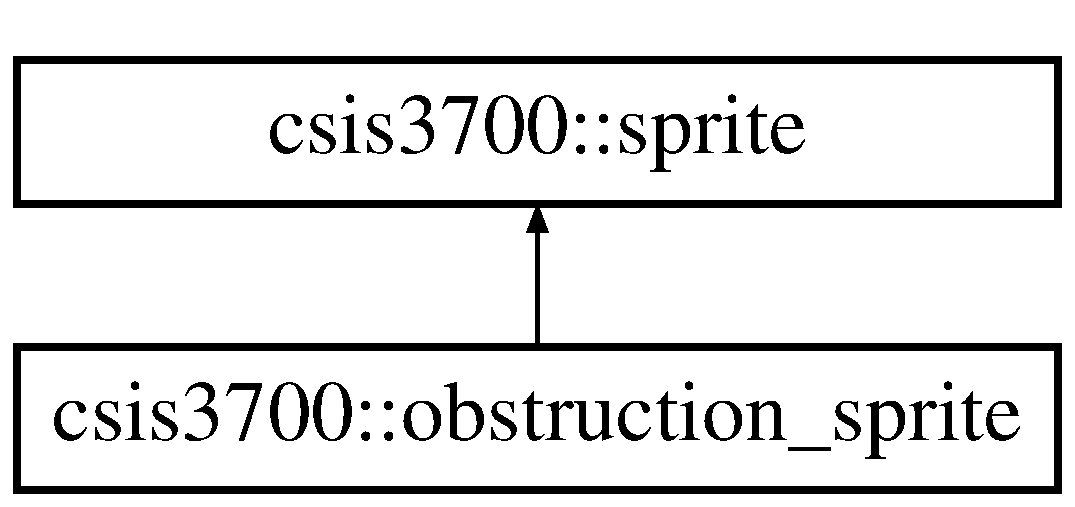
\includegraphics[height=2.000000cm]{classcsis3700_1_1obstruction__sprite}
\end{center}
\end{figure}
\subsection*{Public Member Functions}
\begin{DoxyCompactItemize}
\item 
\mbox{\Hypertarget{classcsis3700_1_1obstruction__sprite_a9d7f66afeeb3dba404c602b54eeb3308}\label{classcsis3700_1_1obstruction__sprite_a9d7f66afeeb3dba404c602b54eeb3308}} 
{\bfseries obstruction\+\_\+sprite} (float initial\+\_\+x, float initial\+\_\+y, A\+L\+L\+E\+G\+R\+O\+\_\+\+B\+I\+T\+M\+AP $\ast$image=N\+U\+LL)
\item 
\mbox{\Hypertarget{classcsis3700_1_1obstruction__sprite_a6629cd0d13f54ed8666326ca55fb7c0c}\label{classcsis3700_1_1obstruction__sprite_a6629cd0d13f54ed8666326ca55fb7c0c}} 
virtual void {\bfseries set\+\_\+velocity} (const \hyperlink{classcsis3700_1_1vec2d}{vec2d} \&v)
\item 
\mbox{\Hypertarget{classcsis3700_1_1obstruction__sprite_aa94cdd034397bd6a30cfe00c15f418ad}\label{classcsis3700_1_1obstruction__sprite_aa94cdd034397bd6a30cfe00c15f418ad}} 
virtual \hyperlink{classcsis3700_1_1vec2d}{vec2d} {\bfseries get\+\_\+velocity} () const
\item 
\mbox{\Hypertarget{classcsis3700_1_1obstruction__sprite_a1ce0b8681cfb6020a332cd97843b4a88}\label{classcsis3700_1_1obstruction__sprite_a1ce0b8681cfb6020a332cd97843b4a88}} 
virtual void {\bfseries resolve} (const \hyperlink{classcsis3700_1_1collision}{collision} \&\hyperlink{classcsis3700_1_1collision}{collision}, \hyperlink{classcsis3700_1_1sprite}{sprite} $\ast$other)
\end{DoxyCompactItemize}
\subsection*{Additional Inherited Members}


\subsection{Detailed Description}
obstruction\+\_\+sprites don\textquotesingle{}t typically move and when they participate in a collision they are unimpacted by it. They typically render themslves as a single, static bitmap. 

The documentation for this class was generated from the following files\+:\begin{DoxyCompactItemize}
\item 
obstruction\+\_\+sprite.\+h\item 
obstruction\+\_\+sprite.\+cpp\end{DoxyCompactItemize}

\hypertarget{classcsis3700_1_1phys__sprite}{}\section{csis3700\+:\+:phys\+\_\+sprite Class Reference}
\label{classcsis3700_1_1phys__sprite}\index{csis3700\+::phys\+\_\+sprite@{csis3700\+::phys\+\_\+sprite}}


{\ttfamily \#include $<$phys\+\_\+sprite.\+h$>$}

Inheritance diagram for csis3700\+:\+:phys\+\_\+sprite\+:\begin{figure}[H]
\begin{center}
\leavevmode
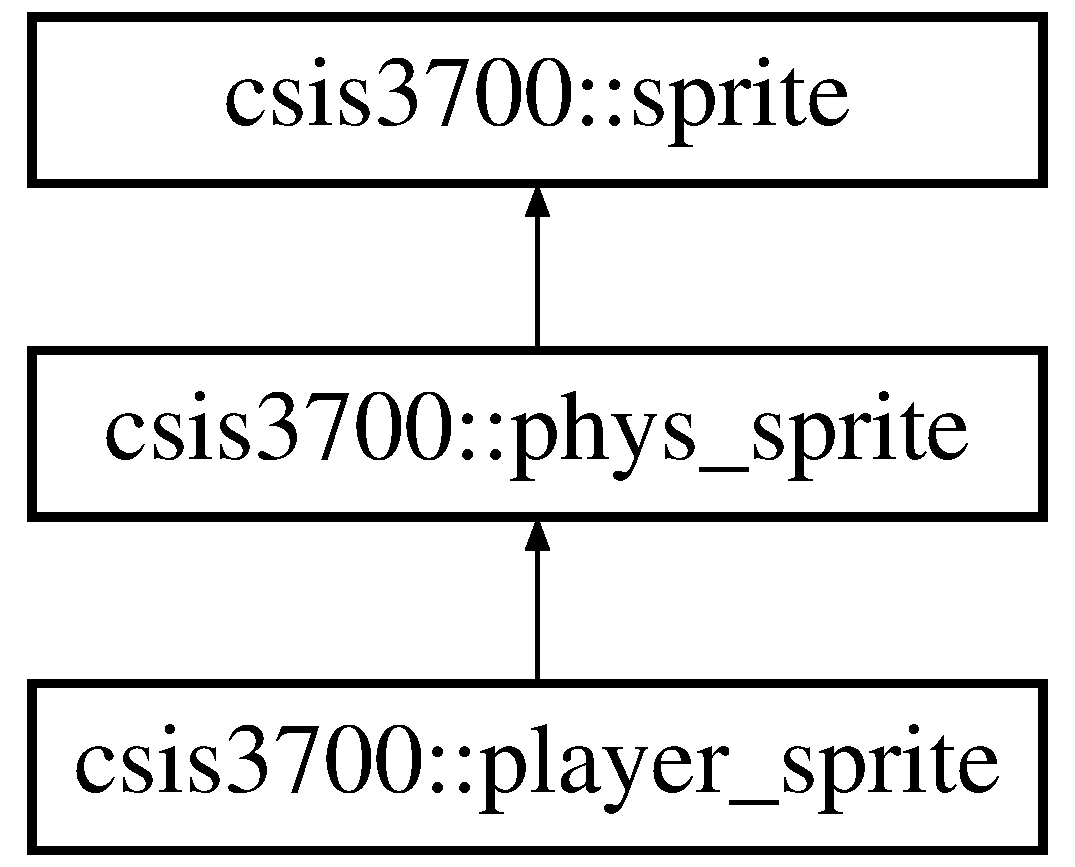
\includegraphics[height=3.000000cm]{classcsis3700_1_1phys__sprite}
\end{center}
\end{figure}
\subsection*{Public Member Functions}
\begin{DoxyCompactItemize}
\item 
\mbox{\Hypertarget{classcsis3700_1_1phys__sprite_a300b8fcf6d18176c9dced92cd90edd99}\label{classcsis3700_1_1phys__sprite_a300b8fcf6d18176c9dced92cd90edd99}} 
{\bfseries phys\+\_\+sprite} (float initial\+\_\+x=0, float initial\+\_\+y=0, float initial\+\_\+vx=0, float initial\+\_\+vy=0)
\item 
virtual void \hyperlink{classcsis3700_1_1phys__sprite_a3bb24599b1bc2fd13846826308914db4}{advance\+\_\+by\+\_\+time} (double dt)
\item 
\mbox{\Hypertarget{classcsis3700_1_1phys__sprite_abfb6a2b73daef8df26dedf0c93e29ec3}\label{classcsis3700_1_1phys__sprite_abfb6a2b73daef8df26dedf0c93e29ec3}} 
virtual \hyperlink{classcsis3700_1_1vec2d}{vec2d} {\bfseries get\+\_\+acceleration} () const
\item 
\mbox{\Hypertarget{classcsis3700_1_1phys__sprite_a91af42ded6d701df0d25ddd08ff70758}\label{classcsis3700_1_1phys__sprite_a91af42ded6d701df0d25ddd08ff70758}} 
virtual \hyperlink{classcsis3700_1_1vec2d}{vec2d} {\bfseries get\+\_\+velocity} () const
\item 
\mbox{\Hypertarget{classcsis3700_1_1phys__sprite_a2dd7b26fd33125f84f3eccabac146dcd}\label{classcsis3700_1_1phys__sprite_a2dd7b26fd33125f84f3eccabac146dcd}} 
virtual void {\bfseries set\+\_\+velocity} (const \hyperlink{classcsis3700_1_1vec2d}{vec2d} \&v)
\item 
\mbox{\Hypertarget{classcsis3700_1_1phys__sprite_ade2d0f1d3e03981d89a8549ec3a1999c}\label{classcsis3700_1_1phys__sprite_ade2d0f1d3e03981d89a8549ec3a1999c}} 
virtual void {\bfseries add\+\_\+force} (\hyperlink{classcsis3700_1_1vec2d}{vec2d} f)
\end{DoxyCompactItemize}
\subsection*{Additional Inherited Members}


\subsection{Detailed Description}
Physical sprites move using an approximation of newtonian kinematics. 

\subsection{Member Function Documentation}
\mbox{\Hypertarget{classcsis3700_1_1phys__sprite_a3bb24599b1bc2fd13846826308914db4}\label{classcsis3700_1_1phys__sprite_a3bb24599b1bc2fd13846826308914db4}} 
\index{csis3700\+::phys\+\_\+sprite@{csis3700\+::phys\+\_\+sprite}!advance\+\_\+by\+\_\+time@{advance\+\_\+by\+\_\+time}}
\index{advance\+\_\+by\+\_\+time@{advance\+\_\+by\+\_\+time}!csis3700\+::phys\+\_\+sprite@{csis3700\+::phys\+\_\+sprite}}
\subsubsection{\texorpdfstring{advance\+\_\+by\+\_\+time()}{advance\_by\_time()}}
{\footnotesize\ttfamily void csis3700\+::phys\+\_\+sprite\+::advance\+\_\+by\+\_\+time (\begin{DoxyParamCaption}\item[{double}]{dt }\end{DoxyParamCaption})\hspace{0.3cm}{\ttfamily [virtual]}}

Move time forward by the specified amount 

Reimplemented from \hyperlink{classcsis3700_1_1sprite_ac4d932bda87ce98a36579de3e1392a8f}{csis3700\+::sprite}.



Reimplemented in \hyperlink{classcsis3700_1_1player__sprite_ac2453e0b3934ac639d704c4ecca7493d}{csis3700\+::player\+\_\+sprite}.



The documentation for this class was generated from the following files\+:\begin{DoxyCompactItemize}
\item 
phys\+\_\+sprite.\+h\item 
phys\+\_\+sprite.\+cpp\end{DoxyCompactItemize}

\hypertarget{classcsis3700_1_1player__sprite}{}\section{csis3700\+:\+:player\+\_\+sprite Class Reference}
\label{classcsis3700_1_1player__sprite}\index{csis3700\+::player\+\_\+sprite@{csis3700\+::player\+\_\+sprite}}
Inheritance diagram for csis3700\+:\+:player\+\_\+sprite\+:\begin{figure}[H]
\begin{center}
\leavevmode
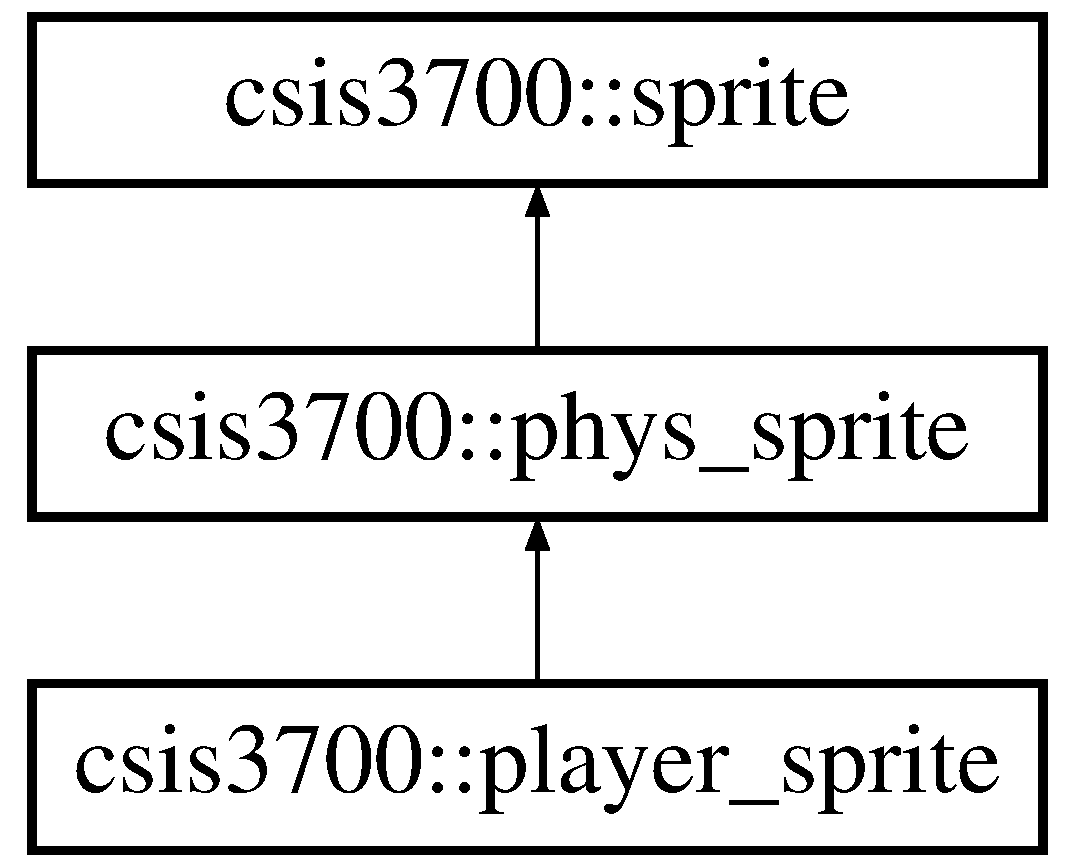
\includegraphics[height=3.000000cm]{classcsis3700_1_1player__sprite}
\end{center}
\end{figure}
\subsection*{Public Member Functions}
\begin{DoxyCompactItemize}
\item 
\mbox{\Hypertarget{classcsis3700_1_1player__sprite_ac187a629d01d5499a19a96e10c132aab}\label{classcsis3700_1_1player__sprite_ac187a629d01d5499a19a96e10c132aab}} 
{\bfseries player\+\_\+sprite} (float initial\+\_\+x=0, float initial\+\_\+y=0)
\item 
\mbox{\Hypertarget{classcsis3700_1_1player__sprite_a4d58637b044853739e75f0e329cb8d67}\label{classcsis3700_1_1player__sprite_a4d58637b044853739e75f0e329cb8d67}} 
virtual bool {\bfseries is\+\_\+passive} () const
\item 
\mbox{\Hypertarget{classcsis3700_1_1player__sprite_a2fc12d698304e7db48bee063e2cde2be}\label{classcsis3700_1_1player__sprite_a2fc12d698304e7db48bee063e2cde2be}} 
virtual void {\bfseries set\+\_\+on\+\_\+ground} (bool v)
\item 
virtual void \hyperlink{classcsis3700_1_1player__sprite_ac2453e0b3934ac639d704c4ecca7493d}{advance\+\_\+by\+\_\+time} (double dt)
\item 
\mbox{\Hypertarget{classcsis3700_1_1player__sprite_a05d3409aa60e9eae24b696c9e9508b7a}\label{classcsis3700_1_1player__sprite_a05d3409aa60e9eae24b696c9e9508b7a}} 
virtual void {\bfseries resolve} (const \hyperlink{classcsis3700_1_1collision}{collision} \&\hyperlink{classcsis3700_1_1collision}{collision}, \hyperlink{classcsis3700_1_1sprite}{sprite} $\ast$other)
\end{DoxyCompactItemize}
\subsection*{Additional Inherited Members}


\subsection{Member Function Documentation}
\mbox{\Hypertarget{classcsis3700_1_1player__sprite_ac2453e0b3934ac639d704c4ecca7493d}\label{classcsis3700_1_1player__sprite_ac2453e0b3934ac639d704c4ecca7493d}} 
\index{csis3700\+::player\+\_\+sprite@{csis3700\+::player\+\_\+sprite}!advance\+\_\+by\+\_\+time@{advance\+\_\+by\+\_\+time}}
\index{advance\+\_\+by\+\_\+time@{advance\+\_\+by\+\_\+time}!csis3700\+::player\+\_\+sprite@{csis3700\+::player\+\_\+sprite}}
\subsubsection{\texorpdfstring{advance\+\_\+by\+\_\+time()}{advance\_by\_time()}}
{\footnotesize\ttfamily void csis3700\+::player\+\_\+sprite\+::advance\+\_\+by\+\_\+time (\begin{DoxyParamCaption}\item[{double}]{dt }\end{DoxyParamCaption})\hspace{0.3cm}{\ttfamily [virtual]}}

Move time forward by the specified amount 

Reimplemented from \hyperlink{classcsis3700_1_1phys__sprite_a3bb24599b1bc2fd13846826308914db4}{csis3700\+::phys\+\_\+sprite}.



The documentation for this class was generated from the following files\+:\begin{DoxyCompactItemize}
\item 
player\+\_\+sprite.\+h\item 
player\+\_\+sprite.\+cpp\end{DoxyCompactItemize}

\hypertarget{classcsis3700_1_1rectangle}{}\section{csis3700\+:\+:rectangle Class Reference}
\label{classcsis3700_1_1rectangle}\index{csis3700\+::rectangle@{csis3700\+::rectangle}}


{\ttfamily \#include $<$rectangle.\+h$>$}

\subsection*{Public Member Functions}
\begin{DoxyCompactItemize}
\item 
\hyperlink{classcsis3700_1_1rectangle_a12769987479c35eb82d4c327c5af31fb}{rectangle} (float x, float y, float width, float height)
\item 
\hyperlink{classcsis3700_1_1rectangle_a343355b4f013ac440b155d634ebc1c5c}{rectangle} (\hyperlink{classcsis3700_1_1vec2d}{vec2d} corner, float width, float height)
\item 
\hyperlink{classcsis3700_1_1rectangle_a65e217f0a67f76c2014b34f5995c689d}{rectangle} (\hyperlink{classcsis3700_1_1vec2d}{vec2d} \hyperlink{classcsis3700_1_1rectangle_a8d1b0714f3e711e5aaa6b708d358b945}{upper\+\_\+left\+\_\+corner}, \hyperlink{classcsis3700_1_1vec2d}{vec2d} \hyperlink{classcsis3700_1_1rectangle_af54b1619b62550375df6a272b25c96b6}{lower\+\_\+right\+\_\+corner})
\item 
\mbox{\Hypertarget{classcsis3700_1_1rectangle_acf6f6686418d6c645704cadee57d6e83}\label{classcsis3700_1_1rectangle_acf6f6686418d6c645704cadee57d6e83}} 
float {\bfseries get\+\_\+width} () const
\item 
\mbox{\Hypertarget{classcsis3700_1_1rectangle_a019b442975cc327d4693c214edfe15c4}\label{classcsis3700_1_1rectangle_a019b442975cc327d4693c214edfe15c4}} 
float {\bfseries get\+\_\+height} () const
\item 
\mbox{\Hypertarget{classcsis3700_1_1rectangle_ab8a18ef5682e35b877600c3051d580c2}\label{classcsis3700_1_1rectangle_ab8a18ef5682e35b877600c3051d580c2}} 
float {\bfseries get\+\_\+area} () const
\item 
\hyperlink{classcsis3700_1_1vec2d}{vec2d} \hyperlink{classcsis3700_1_1rectangle_a8d1b0714f3e711e5aaa6b708d358b945}{upper\+\_\+left\+\_\+corner} () const
\item 
\hyperlink{classcsis3700_1_1vec2d}{vec2d} \hyperlink{classcsis3700_1_1rectangle_af54b1619b62550375df6a272b25c96b6}{lower\+\_\+right\+\_\+corner} () const
\item 
\hyperlink{classcsis3700_1_1rectangle}{rectangle} \hyperlink{classcsis3700_1_1rectangle_ae6306167ac675bdf07cf3a834f1148ae}{intersection} (const \hyperlink{classcsis3700_1_1rectangle}{rectangle} \&other) const
\item 
bool \hyperlink{classcsis3700_1_1rectangle_a15d2ad3f67159bd7724a3728203b1f29}{contains} (\hyperlink{classcsis3700_1_1vec2d}{vec2d} point) const
\item 
bool \hyperlink{classcsis3700_1_1rectangle_a8d897bc040bd296de7206a0576189dc6}{is\+\_\+degenerate} () const
\end{DoxyCompactItemize}


\subsection{Detailed Description}
I represent an oriented rectangle. My sides are parallel to the x and y axes of the coordinate system. 

\subsection{Constructor \& Destructor Documentation}
\mbox{\Hypertarget{classcsis3700_1_1rectangle_a12769987479c35eb82d4c327c5af31fb}\label{classcsis3700_1_1rectangle_a12769987479c35eb82d4c327c5af31fb}} 
\index{csis3700\+::rectangle@{csis3700\+::rectangle}!rectangle@{rectangle}}
\index{rectangle@{rectangle}!csis3700\+::rectangle@{csis3700\+::rectangle}}
\subsubsection{\texorpdfstring{rectangle()}{rectangle()}\hspace{0.1cm}{\footnotesize\ttfamily [1/3]}}
{\footnotesize\ttfamily csis3700\+::rectangle\+::rectangle (\begin{DoxyParamCaption}\item[{float}]{x,  }\item[{float}]{y,  }\item[{float}]{width,  }\item[{float}]{height }\end{DoxyParamCaption})}

Construct a rectangle. Note if width or height is negative then this rectangle is considered degenerate (empty). \mbox{\Hypertarget{classcsis3700_1_1rectangle_a343355b4f013ac440b155d634ebc1c5c}\label{classcsis3700_1_1rectangle_a343355b4f013ac440b155d634ebc1c5c}} 
\index{csis3700\+::rectangle@{csis3700\+::rectangle}!rectangle@{rectangle}}
\index{rectangle@{rectangle}!csis3700\+::rectangle@{csis3700\+::rectangle}}
\subsubsection{\texorpdfstring{rectangle()}{rectangle()}\hspace{0.1cm}{\footnotesize\ttfamily [2/3]}}
{\footnotesize\ttfamily csis3700\+::rectangle\+::rectangle (\begin{DoxyParamCaption}\item[{\hyperlink{classcsis3700_1_1vec2d}{vec2d}}]{corner,  }\item[{float}]{width,  }\item[{float}]{height }\end{DoxyParamCaption})}

Construct a rectangle by specifying the position of its upper left corner as well as its dimensions. \mbox{\Hypertarget{classcsis3700_1_1rectangle_a65e217f0a67f76c2014b34f5995c689d}\label{classcsis3700_1_1rectangle_a65e217f0a67f76c2014b34f5995c689d}} 
\index{csis3700\+::rectangle@{csis3700\+::rectangle}!rectangle@{rectangle}}
\index{rectangle@{rectangle}!csis3700\+::rectangle@{csis3700\+::rectangle}}
\subsubsection{\texorpdfstring{rectangle()}{rectangle()}\hspace{0.1cm}{\footnotesize\ttfamily [3/3]}}
{\footnotesize\ttfamily csis3700\+::rectangle\+::rectangle (\begin{DoxyParamCaption}\item[{\hyperlink{classcsis3700_1_1vec2d}{vec2d}}]{upper\+\_\+left\+\_\+corner,  }\item[{\hyperlink{classcsis3700_1_1vec2d}{vec2d}}]{lower\+\_\+right\+\_\+corner }\end{DoxyParamCaption})}

Construct a rectangle given two corners. The order of the corners is important. upper\+\_\+left\+\_\+corner must be above and to the left of lower\+\_\+right\+\_\+corner or the rectangle will be degenerate. Note orientation is in terms of typical graphical coordinates (increasing y is down). 

\subsection{Member Function Documentation}
\mbox{\Hypertarget{classcsis3700_1_1rectangle_a15d2ad3f67159bd7724a3728203b1f29}\label{classcsis3700_1_1rectangle_a15d2ad3f67159bd7724a3728203b1f29}} 
\index{csis3700\+::rectangle@{csis3700\+::rectangle}!contains@{contains}}
\index{contains@{contains}!csis3700\+::rectangle@{csis3700\+::rectangle}}
\subsubsection{\texorpdfstring{contains()}{contains()}}
{\footnotesize\ttfamily bool csis3700\+::rectangle\+::contains (\begin{DoxyParamCaption}\item[{\hyperlink{classcsis3700_1_1vec2d}{vec2d}}]{point }\end{DoxyParamCaption}) const}

Returns true iff this rectangle contains the point specified by the supplied vector (relative to the origin). \mbox{\Hypertarget{classcsis3700_1_1rectangle_ae6306167ac675bdf07cf3a834f1148ae}\label{classcsis3700_1_1rectangle_ae6306167ac675bdf07cf3a834f1148ae}} 
\index{csis3700\+::rectangle@{csis3700\+::rectangle}!intersection@{intersection}}
\index{intersection@{intersection}!csis3700\+::rectangle@{csis3700\+::rectangle}}
\subsubsection{\texorpdfstring{intersection()}{intersection()}}
{\footnotesize\ttfamily \hyperlink{classcsis3700_1_1rectangle}{rectangle} csis3700\+::rectangle\+::intersection (\begin{DoxyParamCaption}\item[{const \hyperlink{classcsis3700_1_1rectangle}{rectangle} \&}]{other }\end{DoxyParamCaption}) const}

Return the rectangle representing the intersection (overlap) between this rectangle and other. If I do not intersect other, return a degenerate rectangle. \mbox{\Hypertarget{classcsis3700_1_1rectangle_a8d897bc040bd296de7206a0576189dc6}\label{classcsis3700_1_1rectangle_a8d897bc040bd296de7206a0576189dc6}} 
\index{csis3700\+::rectangle@{csis3700\+::rectangle}!is\+\_\+degenerate@{is\+\_\+degenerate}}
\index{is\+\_\+degenerate@{is\+\_\+degenerate}!csis3700\+::rectangle@{csis3700\+::rectangle}}
\subsubsection{\texorpdfstring{is\+\_\+degenerate()}{is\_degenerate()}}
{\footnotesize\ttfamily bool csis3700\+::rectangle\+::is\+\_\+degenerate (\begin{DoxyParamCaption}{ }\end{DoxyParamCaption}) const}

Return true if this rectangle is degenerate. A degenerate rectangle is one with negative width or height. \mbox{\Hypertarget{classcsis3700_1_1rectangle_af54b1619b62550375df6a272b25c96b6}\label{classcsis3700_1_1rectangle_af54b1619b62550375df6a272b25c96b6}} 
\index{csis3700\+::rectangle@{csis3700\+::rectangle}!lower\+\_\+right\+\_\+corner@{lower\+\_\+right\+\_\+corner}}
\index{lower\+\_\+right\+\_\+corner@{lower\+\_\+right\+\_\+corner}!csis3700\+::rectangle@{csis3700\+::rectangle}}
\subsubsection{\texorpdfstring{lower\+\_\+right\+\_\+corner()}{lower\_right\_corner()}}
{\footnotesize\ttfamily \hyperlink{classcsis3700_1_1vec2d}{vec2d} csis3700\+::rectangle\+::lower\+\_\+right\+\_\+corner (\begin{DoxyParamCaption}{ }\end{DoxyParamCaption}) const}

Return my lower right corner \mbox{\Hypertarget{classcsis3700_1_1rectangle_a8d1b0714f3e711e5aaa6b708d358b945}\label{classcsis3700_1_1rectangle_a8d1b0714f3e711e5aaa6b708d358b945}} 
\index{csis3700\+::rectangle@{csis3700\+::rectangle}!upper\+\_\+left\+\_\+corner@{upper\+\_\+left\+\_\+corner}}
\index{upper\+\_\+left\+\_\+corner@{upper\+\_\+left\+\_\+corner}!csis3700\+::rectangle@{csis3700\+::rectangle}}
\subsubsection{\texorpdfstring{upper\+\_\+left\+\_\+corner()}{upper\_left\_corner()}}
{\footnotesize\ttfamily \hyperlink{classcsis3700_1_1vec2d}{vec2d} csis3700\+::rectangle\+::upper\+\_\+left\+\_\+corner (\begin{DoxyParamCaption}{ }\end{DoxyParamCaption}) const}

Return my upper left corner 

The documentation for this class was generated from the following files\+:\begin{DoxyCompactItemize}
\item 
rectangle.\+h\item 
rectangle.\+cpp\end{DoxyCompactItemize}

\hypertarget{classcsis3700_1_1sprite}{}\section{csis3700\+:\+:sprite Class Reference}
\label{classcsis3700_1_1sprite}\index{csis3700\+::sprite@{csis3700\+::sprite}}
Inheritance diagram for csis3700\+:\+:sprite\+:\begin{figure}[H]
\begin{center}
\leavevmode
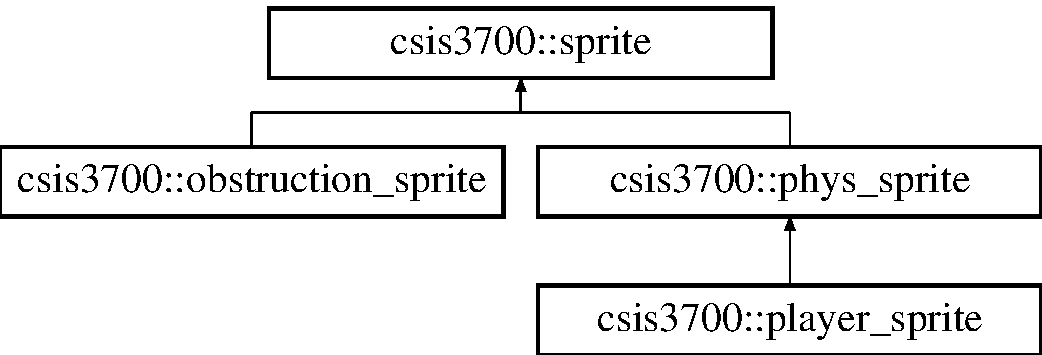
\includegraphics[height=3.000000cm]{classcsis3700_1_1sprite}
\end{center}
\end{figure}
\subsection*{Public Member Functions}
\begin{DoxyCompactItemize}
\item 
\mbox{\Hypertarget{classcsis3700_1_1sprite_a5395ad1b481e56895f11d57c7a052353}\label{classcsis3700_1_1sprite_a5395ad1b481e56895f11d57c7a052353}} 
{\bfseries sprite} (float initial\+\_\+x, float initial\+\_\+y)
\item 
\mbox{\Hypertarget{classcsis3700_1_1sprite_a0b6e3ec9733f1300aac47ecf8570ee0b}\label{classcsis3700_1_1sprite_a0b6e3ec9733f1300aac47ecf8570ee0b}} 
void {\bfseries set\+\_\+image\+\_\+sequence} (\hyperlink{classcsis3700_1_1image__sequence}{image\+\_\+sequence} $\ast$s)
\item 
virtual \hyperlink{classcsis3700_1_1sprite_a8f6db48ecf33279af2d084a344baae8c}{$\sim$sprite} ()
\item 
\hyperlink{classcsis3700_1_1sprite_adff79f206ea0703727a72287242fd8b1}{sprite} (const \hyperlink{classcsis3700_1_1sprite}{sprite} \&other)
\item 
\mbox{\Hypertarget{classcsis3700_1_1sprite_abd31e459d917f4789dd203730144e19a}\label{classcsis3700_1_1sprite_abd31e459d917f4789dd203730144e19a}} 
\hyperlink{classcsis3700_1_1sprite}{sprite} \& {\bfseries operator=} (const \hyperlink{classcsis3700_1_1sprite}{sprite} \&other)
\item 
\mbox{\Hypertarget{classcsis3700_1_1sprite_a8370bcf8a127a7cb240a085400cac95d}\label{classcsis3700_1_1sprite_a8370bcf8a127a7cb240a085400cac95d}} 
virtual int {\bfseries get\+\_\+width} () const
\item 
\mbox{\Hypertarget{classcsis3700_1_1sprite_a9883c2534640adab14fe8594ba4b4f33}\label{classcsis3700_1_1sprite_a9883c2534640adab14fe8594ba4b4f33}} 
virtual int {\bfseries get\+\_\+height} () const
\item 
\mbox{\Hypertarget{classcsis3700_1_1sprite_af70f95b93fe418307c3ec9b95c97e899}\label{classcsis3700_1_1sprite_af70f95b93fe418307c3ec9b95c97e899}} 
virtual float {\bfseries get\+\_\+x} () const
\item 
\mbox{\Hypertarget{classcsis3700_1_1sprite_a2b9c0912475c1d42cf4204591d2ecf1b}\label{classcsis3700_1_1sprite_a2b9c0912475c1d42cf4204591d2ecf1b}} 
virtual float {\bfseries get\+\_\+y} () const
\item 
\mbox{\Hypertarget{classcsis3700_1_1sprite_a2678deb93962cd15eeac659532066d78}\label{classcsis3700_1_1sprite_a2678deb93962cd15eeac659532066d78}} 
virtual \hyperlink{classcsis3700_1_1vec2d}{vec2d} {\bfseries get\+\_\+position} () const
\item 
\mbox{\Hypertarget{classcsis3700_1_1sprite_a433b1dbe4695990e42490d12d1bfac68}\label{classcsis3700_1_1sprite_a433b1dbe4695990e42490d12d1bfac68}} 
virtual void {\bfseries set\+\_\+position} (\hyperlink{classcsis3700_1_1vec2d}{vec2d} p)
\item 
\mbox{\Hypertarget{classcsis3700_1_1sprite_a947c4b01559cbcd9c4dffbc6b39c6fbf}\label{classcsis3700_1_1sprite_a947c4b01559cbcd9c4dffbc6b39c6fbf}} 
virtual \hyperlink{classcsis3700_1_1vec2d}{vec2d} {\bfseries get\+\_\+velocity} () const =0
\item 
\mbox{\Hypertarget{classcsis3700_1_1sprite_a3c43d72d94f5428d06d6f01b8753abe9}\label{classcsis3700_1_1sprite_a3c43d72d94f5428d06d6f01b8753abe9}} 
virtual void {\bfseries set\+\_\+velocity} (const \hyperlink{classcsis3700_1_1vec2d}{vec2d} \&v)=0
\item 
\mbox{\Hypertarget{classcsis3700_1_1sprite_a498d7ab34e5f0367b34ac8355a6b428f}\label{classcsis3700_1_1sprite_a498d7ab34e5f0367b34ac8355a6b428f}} 
virtual bool {\bfseries is\+\_\+passive} () const
\item 
virtual void \hyperlink{classcsis3700_1_1sprite_a6a69657522664635f116e05648792555}{draw} ()
\item 
virtual bool \hyperlink{classcsis3700_1_1sprite_ac3092a26409694577c92ba6d9831c90a}{collides\+\_\+with} (const \hyperlink{classcsis3700_1_1sprite}{sprite} \&other) const
\item 
virtual void \hyperlink{classcsis3700_1_1sprite_ac4d932bda87ce98a36579de3e1392a8f}{advance\+\_\+by\+\_\+time} (double dt)
\item 
virtual \hyperlink{classcsis3700_1_1rectangle}{rectangle} \hyperlink{classcsis3700_1_1sprite_a2ff6edefbdab7f1b49366bed16bfa6e5}{bounding\+\_\+box} () const
\item 
virtual \hyperlink{classcsis3700_1_1rectangle}{rectangle} \hyperlink{classcsis3700_1_1sprite_a54b72f8172133a7099ea2c73db23b4b2}{collision\+\_\+rectangle} (const \hyperlink{classcsis3700_1_1sprite}{sprite} \&other) const
\item 
\mbox{\Hypertarget{classcsis3700_1_1sprite_a4bf20253e1bc1825bfe73cdfcbb532d2}\label{classcsis3700_1_1sprite_a4bf20253e1bc1825bfe73cdfcbb532d2}} 
virtual void {\bfseries resolve} (const \hyperlink{classcsis3700_1_1collision}{collision} \&\hyperlink{classcsis3700_1_1collision}{collision}, \hyperlink{classcsis3700_1_1sprite}{sprite} $\ast$other)=0
\end{DoxyCompactItemize}
\subsection*{Protected Attributes}
\begin{DoxyCompactItemize}
\item 
\hyperlink{classcsis3700_1_1vec2d}{vec2d} \hyperlink{classcsis3700_1_1sprite_aab9ac03c13c18eca432f5db06a8383b8}{position}
\item 
\hyperlink{classcsis3700_1_1image__sequence}{image\+\_\+sequence} $\ast$ \hyperlink{classcsis3700_1_1sprite_aa65b73f9bf7d266e57236f5b606b36e1}{sequence}
\item 
double \hyperlink{classcsis3700_1_1sprite_af12d2211006b3a184af6b70ed9e4235a}{time}
\end{DoxyCompactItemize}


\subsection{Constructor \& Destructor Documentation}
\mbox{\Hypertarget{classcsis3700_1_1sprite_a8f6db48ecf33279af2d084a344baae8c}\label{classcsis3700_1_1sprite_a8f6db48ecf33279af2d084a344baae8c}} 
\index{csis3700\+::sprite@{csis3700\+::sprite}!````~sprite@{$\sim$sprite}}
\index{````~sprite@{$\sim$sprite}!csis3700\+::sprite@{csis3700\+::sprite}}
\subsubsection{\texorpdfstring{$\sim$sprite()}{~sprite()}}
{\footnotesize\ttfamily csis3700\+::sprite\+::$\sim$sprite (\begin{DoxyParamCaption}{ }\end{DoxyParamCaption})\hspace{0.3cm}{\ttfamily [virtual]}}

Destructor \mbox{\Hypertarget{classcsis3700_1_1sprite_adff79f206ea0703727a72287242fd8b1}\label{classcsis3700_1_1sprite_adff79f206ea0703727a72287242fd8b1}} 
\index{csis3700\+::sprite@{csis3700\+::sprite}!sprite@{sprite}}
\index{sprite@{sprite}!csis3700\+::sprite@{csis3700\+::sprite}}
\subsubsection{\texorpdfstring{sprite()}{sprite()}}
{\footnotesize\ttfamily csis3700\+::sprite\+::sprite (\begin{DoxyParamCaption}\item[{const \hyperlink{classcsis3700_1_1sprite}{sprite} \&}]{other }\end{DoxyParamCaption})\hspace{0.3cm}{\ttfamily [inline]}}

these two should cause errors, no copying! 

\subsection{Member Function Documentation}
\mbox{\Hypertarget{classcsis3700_1_1sprite_ac4d932bda87ce98a36579de3e1392a8f}\label{classcsis3700_1_1sprite_ac4d932bda87ce98a36579de3e1392a8f}} 
\index{csis3700\+::sprite@{csis3700\+::sprite}!advance\+\_\+by\+\_\+time@{advance\+\_\+by\+\_\+time}}
\index{advance\+\_\+by\+\_\+time@{advance\+\_\+by\+\_\+time}!csis3700\+::sprite@{csis3700\+::sprite}}
\subsubsection{\texorpdfstring{advance\+\_\+by\+\_\+time()}{advance\_by\_time()}}
{\footnotesize\ttfamily void csis3700\+::sprite\+::advance\+\_\+by\+\_\+time (\begin{DoxyParamCaption}\item[{double}]{dt }\end{DoxyParamCaption})\hspace{0.3cm}{\ttfamily [virtual]}}

Move time forward by the specified amount 

Reimplemented in \hyperlink{classcsis3700_1_1phys__sprite_a3bb24599b1bc2fd13846826308914db4}{csis3700\+::phys\+\_\+sprite}, and \hyperlink{classcsis3700_1_1player__sprite_ac2453e0b3934ac639d704c4ecca7493d}{csis3700\+::player\+\_\+sprite}.

\mbox{\Hypertarget{classcsis3700_1_1sprite_a2ff6edefbdab7f1b49366bed16bfa6e5}\label{classcsis3700_1_1sprite_a2ff6edefbdab7f1b49366bed16bfa6e5}} 
\index{csis3700\+::sprite@{csis3700\+::sprite}!bounding\+\_\+box@{bounding\+\_\+box}}
\index{bounding\+\_\+box@{bounding\+\_\+box}!csis3700\+::sprite@{csis3700\+::sprite}}
\subsubsection{\texorpdfstring{bounding\+\_\+box()}{bounding\_box()}}
{\footnotesize\ttfamily \hyperlink{classcsis3700_1_1rectangle}{rectangle} csis3700\+::sprite\+::bounding\+\_\+box (\begin{DoxyParamCaption}{ }\end{DoxyParamCaption}) const\hspace{0.3cm}{\ttfamily [virtual]}}

Return this sprite\textquotesingle{}s bounding box \mbox{\Hypertarget{classcsis3700_1_1sprite_ac3092a26409694577c92ba6d9831c90a}\label{classcsis3700_1_1sprite_ac3092a26409694577c92ba6d9831c90a}} 
\index{csis3700\+::sprite@{csis3700\+::sprite}!collides\+\_\+with@{collides\+\_\+with}}
\index{collides\+\_\+with@{collides\+\_\+with}!csis3700\+::sprite@{csis3700\+::sprite}}
\subsubsection{\texorpdfstring{collides\+\_\+with()}{collides\_with()}}
{\footnotesize\ttfamily bool csis3700\+::sprite\+::collides\+\_\+with (\begin{DoxyParamCaption}\item[{const \hyperlink{classcsis3700_1_1sprite}{sprite} \&}]{other }\end{DoxyParamCaption}) const\hspace{0.3cm}{\ttfamily [virtual]}}

Returns true iff I collide with other. Default implementation returns true iff my bounding box overlaps other\textquotesingle{}s. \mbox{\Hypertarget{classcsis3700_1_1sprite_a54b72f8172133a7099ea2c73db23b4b2}\label{classcsis3700_1_1sprite_a54b72f8172133a7099ea2c73db23b4b2}} 
\index{csis3700\+::sprite@{csis3700\+::sprite}!collision\+\_\+rectangle@{collision\+\_\+rectangle}}
\index{collision\+\_\+rectangle@{collision\+\_\+rectangle}!csis3700\+::sprite@{csis3700\+::sprite}}
\subsubsection{\texorpdfstring{collision\+\_\+rectangle()}{collision\_rectangle()}}
{\footnotesize\ttfamily \hyperlink{classcsis3700_1_1rectangle}{rectangle} csis3700\+::sprite\+::collision\+\_\+rectangle (\begin{DoxyParamCaption}\item[{const \hyperlink{classcsis3700_1_1sprite}{sprite} \&}]{other }\end{DoxyParamCaption}) const\hspace{0.3cm}{\ttfamily [virtual]}}

Return the intersection of this sprite\textquotesingle{}s bounding box with other\textquotesingle{}s bounding box. \mbox{\Hypertarget{classcsis3700_1_1sprite_a6a69657522664635f116e05648792555}\label{classcsis3700_1_1sprite_a6a69657522664635f116e05648792555}} 
\index{csis3700\+::sprite@{csis3700\+::sprite}!draw@{draw}}
\index{draw@{draw}!csis3700\+::sprite@{csis3700\+::sprite}}
\subsubsection{\texorpdfstring{draw()}{draw()}}
{\footnotesize\ttfamily void csis3700\+::sprite\+::draw (\begin{DoxyParamCaption}{ }\end{DoxyParamCaption})\hspace{0.3cm}{\ttfamily [virtual]}}

Draw this sprite. 

\subsection{Member Data Documentation}
\mbox{\Hypertarget{classcsis3700_1_1sprite_aab9ac03c13c18eca432f5db06a8383b8}\label{classcsis3700_1_1sprite_aab9ac03c13c18eca432f5db06a8383b8}} 
\index{csis3700\+::sprite@{csis3700\+::sprite}!position@{position}}
\index{position@{position}!csis3700\+::sprite@{csis3700\+::sprite}}
\subsubsection{\texorpdfstring{position}{position}}
{\footnotesize\ttfamily \hyperlink{classcsis3700_1_1vec2d}{vec2d} csis3700\+::sprite\+::position\hspace{0.3cm}{\ttfamily [protected]}}

My position \mbox{\Hypertarget{classcsis3700_1_1sprite_aa65b73f9bf7d266e57236f5b606b36e1}\label{classcsis3700_1_1sprite_aa65b73f9bf7d266e57236f5b606b36e1}} 
\index{csis3700\+::sprite@{csis3700\+::sprite}!sequence@{sequence}}
\index{sequence@{sequence}!csis3700\+::sprite@{csis3700\+::sprite}}
\subsubsection{\texorpdfstring{sequence}{sequence}}
{\footnotesize\ttfamily \hyperlink{classcsis3700_1_1image__sequence}{image\+\_\+sequence}$\ast$ csis3700\+::sprite\+::sequence\hspace{0.3cm}{\ttfamily [protected]}}

My current image sequence \mbox{\Hypertarget{classcsis3700_1_1sprite_af12d2211006b3a184af6b70ed9e4235a}\label{classcsis3700_1_1sprite_af12d2211006b3a184af6b70ed9e4235a}} 
\index{csis3700\+::sprite@{csis3700\+::sprite}!time@{time}}
\index{time@{time}!csis3700\+::sprite@{csis3700\+::sprite}}
\subsubsection{\texorpdfstring{time}{time}}
{\footnotesize\ttfamily double csis3700\+::sprite\+::time\hspace{0.3cm}{\ttfamily [protected]}}

The time in seconds since the world began ticking 

The documentation for this class was generated from the following files\+:\begin{DoxyCompactItemize}
\item 
sprite.\+h\item 
sprite.\+cpp\end{DoxyCompactItemize}

\hypertarget{classcsis3700_1_1vec2d}{}\section{csis3700\+:\+:vec2d Class Reference}
\label{classcsis3700_1_1vec2d}\index{csis3700\+::vec2d@{csis3700\+::vec2d}}


{\ttfamily \#include $<$vec2d.\+h$>$}

\subsection*{Public Member Functions}
\begin{DoxyCompactItemize}
\item 
\mbox{\Hypertarget{classcsis3700_1_1vec2d_a40ee61b39f4e735dc12bd6030036c276}\label{classcsis3700_1_1vec2d_a40ee61b39f4e735dc12bd6030036c276}} 
{\bfseries vec2d} (float initial\+\_\+x=0, float initial\+\_\+y=0)
\item 
\mbox{\Hypertarget{classcsis3700_1_1vec2d_abbc06aa198f2a0c974259e3e08a7bc09}\label{classcsis3700_1_1vec2d_abbc06aa198f2a0c974259e3e08a7bc09}} 
float {\bfseries get\+\_\+x} () const
\item 
\mbox{\Hypertarget{classcsis3700_1_1vec2d_aa9d00524399eccfa186fb19b5cf9e635}\label{classcsis3700_1_1vec2d_aa9d00524399eccfa186fb19b5cf9e635}} 
float {\bfseries get\+\_\+y} () const
\item 
\hyperlink{classcsis3700_1_1vec2d}{vec2d} \hyperlink{classcsis3700_1_1vec2d_af0b6fa5ce2a480ad9d0c4ab1fbbe4d1b}{operator+} (const \hyperlink{classcsis3700_1_1vec2d}{vec2d} \&other) const
\item 
\hyperlink{classcsis3700_1_1vec2d}{vec2d} \hyperlink{classcsis3700_1_1vec2d_a423878a90a2ea8ac8174f4b8d9b2721e}{operator-\/} (const \hyperlink{classcsis3700_1_1vec2d}{vec2d} \&other) const
\item 
bool \hyperlink{classcsis3700_1_1vec2d_a03dc593f880647772abb9b0abc865cbe}{operator==} (const \hyperlink{classcsis3700_1_1vec2d}{vec2d} \&other) const
\item 
\hyperlink{classcsis3700_1_1vec2d}{vec2d} \hyperlink{classcsis3700_1_1vec2d_ac311938a3cf00e5cd919e27493337ed1}{max} (const \hyperlink{classcsis3700_1_1vec2d}{vec2d} \&other) const
\item 
\hyperlink{classcsis3700_1_1vec2d}{vec2d} \hyperlink{classcsis3700_1_1vec2d_a6368f4e6d0d7031278b540a5dda5bb91}{min} (const \hyperlink{classcsis3700_1_1vec2d}{vec2d} \&other) const
\item 
\hyperlink{classcsis3700_1_1vec2d}{vec2d} \hyperlink{classcsis3700_1_1vec2d_a73b3a12f9c2ebddb35d6cda11e167964}{clamp} (float max\+\_\+x, float max\+\_\+y) const
\item 
\mbox{\Hypertarget{classcsis3700_1_1vec2d_a2dc8b8021ffeed353db058f4815c8c24}\label{classcsis3700_1_1vec2d_a2dc8b8021ffeed353db058f4815c8c24}} 
\hyperlink{classcsis3700_1_1vec2d}{vec2d} \& {\bfseries operator+=} (const \hyperlink{classcsis3700_1_1vec2d}{vec2d} \&other)
\end{DoxyCompactItemize}


\subsection{Detailed Description}
A 2-\/dimensional vector. Also used for point-\/like operations in which case, as a point, this vector is interpreted as the point corresponding to its endpoint if it began at the origin (that is a point with coordinates (x,y)). 

\subsection{Member Function Documentation}
\mbox{\Hypertarget{classcsis3700_1_1vec2d_a73b3a12f9c2ebddb35d6cda11e167964}\label{classcsis3700_1_1vec2d_a73b3a12f9c2ebddb35d6cda11e167964}} 
\index{csis3700\+::vec2d@{csis3700\+::vec2d}!clamp@{clamp}}
\index{clamp@{clamp}!csis3700\+::vec2d@{csis3700\+::vec2d}}
\subsubsection{\texorpdfstring{clamp()}{clamp()}}
{\footnotesize\ttfamily \hyperlink{classcsis3700_1_1vec2d}{vec2d} csis3700\+::vec2d\+::clamp (\begin{DoxyParamCaption}\item[{float}]{max\+\_\+x,  }\item[{float}]{max\+\_\+y }\end{DoxyParamCaption}) const}

Return a vector whose x component is between -\/max\+\_\+x and max\+\_\+x and whose y component is between -\/max\+\_\+y and max\+\_\+y. If the condition on the component is already met, do nothing to it, otherwise set it to the max with the appropriate sign. \mbox{\Hypertarget{classcsis3700_1_1vec2d_ac311938a3cf00e5cd919e27493337ed1}\label{classcsis3700_1_1vec2d_ac311938a3cf00e5cd919e27493337ed1}} 
\index{csis3700\+::vec2d@{csis3700\+::vec2d}!max@{max}}
\index{max@{max}!csis3700\+::vec2d@{csis3700\+::vec2d}}
\subsubsection{\texorpdfstring{max()}{max()}}
{\footnotesize\ttfamily \hyperlink{classcsis3700_1_1vec2d}{vec2d} csis3700\+::vec2d\+::max (\begin{DoxyParamCaption}\item[{const \hyperlink{classcsis3700_1_1vec2d}{vec2d} \&}]{other }\end{DoxyParamCaption}) const}

Return a vector whose x is the max of this.\+x and other.\+x and whose y is the max of this.\+y and other.\+y. \mbox{\Hypertarget{classcsis3700_1_1vec2d_a6368f4e6d0d7031278b540a5dda5bb91}\label{classcsis3700_1_1vec2d_a6368f4e6d0d7031278b540a5dda5bb91}} 
\index{csis3700\+::vec2d@{csis3700\+::vec2d}!min@{min}}
\index{min@{min}!csis3700\+::vec2d@{csis3700\+::vec2d}}
\subsubsection{\texorpdfstring{min()}{min()}}
{\footnotesize\ttfamily \hyperlink{classcsis3700_1_1vec2d}{vec2d} csis3700\+::vec2d\+::min (\begin{DoxyParamCaption}\item[{const \hyperlink{classcsis3700_1_1vec2d}{vec2d} \&}]{other }\end{DoxyParamCaption}) const}

Return a vector whose x is the min of this.\+x and other.\+x and whose y is the min of this.\+y and other.\+y. \mbox{\Hypertarget{classcsis3700_1_1vec2d_af0b6fa5ce2a480ad9d0c4ab1fbbe4d1b}\label{classcsis3700_1_1vec2d_af0b6fa5ce2a480ad9d0c4ab1fbbe4d1b}} 
\index{csis3700\+::vec2d@{csis3700\+::vec2d}!operator+@{operator+}}
\index{operator+@{operator+}!csis3700\+::vec2d@{csis3700\+::vec2d}}
\subsubsection{\texorpdfstring{operator+()}{operator+()}}
{\footnotesize\ttfamily \hyperlink{classcsis3700_1_1vec2d}{vec2d} csis3700\+::vec2d\+::operator+ (\begin{DoxyParamCaption}\item[{const \hyperlink{classcsis3700_1_1vec2d}{vec2d} \&}]{other }\end{DoxyParamCaption}) const}

The vector sum of this and other. \mbox{\Hypertarget{classcsis3700_1_1vec2d_a423878a90a2ea8ac8174f4b8d9b2721e}\label{classcsis3700_1_1vec2d_a423878a90a2ea8ac8174f4b8d9b2721e}} 
\index{csis3700\+::vec2d@{csis3700\+::vec2d}!operator-\/@{operator-\/}}
\index{operator-\/@{operator-\/}!csis3700\+::vec2d@{csis3700\+::vec2d}}
\subsubsection{\texorpdfstring{operator-\/()}{operator-()}}
{\footnotesize\ttfamily \hyperlink{classcsis3700_1_1vec2d}{vec2d} csis3700\+::vec2d\+::operator-\/ (\begin{DoxyParamCaption}\item[{const \hyperlink{classcsis3700_1_1vec2d}{vec2d} \&}]{other }\end{DoxyParamCaption}) const}

The vector difference (this -\/ other) \mbox{\Hypertarget{classcsis3700_1_1vec2d_a03dc593f880647772abb9b0abc865cbe}\label{classcsis3700_1_1vec2d_a03dc593f880647772abb9b0abc865cbe}} 
\index{csis3700\+::vec2d@{csis3700\+::vec2d}!operator==@{operator==}}
\index{operator==@{operator==}!csis3700\+::vec2d@{csis3700\+::vec2d}}
\subsubsection{\texorpdfstring{operator==()}{operator==()}}
{\footnotesize\ttfamily bool csis3700\+::vec2d\+::operator== (\begin{DoxyParamCaption}\item[{const \hyperlink{classcsis3700_1_1vec2d}{vec2d} \&}]{other }\end{DoxyParamCaption}) const}

Two vectors are equal iff their components are exactly equal. Be careful with floats! 

The documentation for this class was generated from the following files\+:\begin{DoxyCompactItemize}
\item 
vec2d.\+h\item 
vec2d.\+cpp\end{DoxyCompactItemize}

\hypertarget{classcsis3700_1_1world}{}\section{csis3700\+:\+:world Class Reference}
\label{classcsis3700_1_1world}\index{csis3700\+::world@{csis3700\+::world}}
\subsection*{Public Member Functions}
\begin{DoxyCompactItemize}
\item 
\hyperlink{classcsis3700_1_1world_add94e82a5e7c88d9f4f2714c199693b1}{world} ()
\item 
\hyperlink{classcsis3700_1_1world_ae793effd77990768c2f7565cb2daba70}{$\sim$world} ()
\item 
\hyperlink{classcsis3700_1_1world_a323fcd5b15ee4a274bffe02cf9c7cd0e}{world} (const \hyperlink{classcsis3700_1_1world}{world} \&other)
\item 
\hyperlink{classcsis3700_1_1world}{world} \& \hyperlink{classcsis3700_1_1world_a1ce9a5a4c2a161b8d0bd079727632d62}{operator=} (const \hyperlink{classcsis3700_1_1world}{world} \&other)
\item 
void \hyperlink{classcsis3700_1_1world_a244cfed1968f6ed5133b82eebcb0c158}{handle\+\_\+event} (A\+L\+L\+E\+G\+R\+O\+\_\+\+E\+V\+E\+NT ev)
\item 
void \hyperlink{classcsis3700_1_1world_a2b4a33cc658001cde9d838ff50237a5f}{advance\+\_\+by\+\_\+time} (double dt)
\item 
void \hyperlink{classcsis3700_1_1world_acd1681a6ac117cf74ac4590938d60a80}{draw} ()
\item 
bool \hyperlink{classcsis3700_1_1world_a72b6c90fa52ae434dc866f40caf5ee07}{should\+\_\+exit} ()
\end{DoxyCompactItemize}


\subsection{Constructor \& Destructor Documentation}
\mbox{\Hypertarget{classcsis3700_1_1world_add94e82a5e7c88d9f4f2714c199693b1}\label{classcsis3700_1_1world_add94e82a5e7c88d9f4f2714c199693b1}} 
\index{csis3700\+::world@{csis3700\+::world}!world@{world}}
\index{world@{world}!csis3700\+::world@{csis3700\+::world}}
\subsubsection{\texorpdfstring{world()}{world()}\hspace{0.1cm}{\footnotesize\ttfamily [1/2]}}
{\footnotesize\ttfamily csis3700\+::world\+::world (\begin{DoxyParamCaption}{ }\end{DoxyParamCaption})}

Construct the world. The display is passed in simply to make it possible to modify options or access the backbuffer. DO N\+OT store the display in an instance variable. DO N\+OT start drawing on the screen. Just load bitmaps etc. \mbox{\Hypertarget{classcsis3700_1_1world_ae793effd77990768c2f7565cb2daba70}\label{classcsis3700_1_1world_ae793effd77990768c2f7565cb2daba70}} 
\index{csis3700\+::world@{csis3700\+::world}!````~world@{$\sim$world}}
\index{````~world@{$\sim$world}!csis3700\+::world@{csis3700\+::world}}
\subsubsection{\texorpdfstring{$\sim$world()}{~world()}}
{\footnotesize\ttfamily csis3700\+::world\+::$\sim$world (\begin{DoxyParamCaption}{ }\end{DoxyParamCaption})}

Free any resources being used by the world. \mbox{\Hypertarget{classcsis3700_1_1world_a323fcd5b15ee4a274bffe02cf9c7cd0e}\label{classcsis3700_1_1world_a323fcd5b15ee4a274bffe02cf9c7cd0e}} 
\index{csis3700\+::world@{csis3700\+::world}!world@{world}}
\index{world@{world}!csis3700\+::world@{csis3700\+::world}}
\subsubsection{\texorpdfstring{world()}{world()}\hspace{0.1cm}{\footnotesize\ttfamily [2/2]}}
{\footnotesize\ttfamily csis3700\+::world\+::world (\begin{DoxyParamCaption}\item[{const \hyperlink{classcsis3700_1_1world}{world} \&}]{other }\end{DoxyParamCaption})}

Block the copy constructor. Worlds should not be copied to just assert(false) 

\subsection{Member Function Documentation}
\mbox{\Hypertarget{classcsis3700_1_1world_a2b4a33cc658001cde9d838ff50237a5f}\label{classcsis3700_1_1world_a2b4a33cc658001cde9d838ff50237a5f}} 
\index{csis3700\+::world@{csis3700\+::world}!advance\+\_\+by\+\_\+time@{advance\+\_\+by\+\_\+time}}
\index{advance\+\_\+by\+\_\+time@{advance\+\_\+by\+\_\+time}!csis3700\+::world@{csis3700\+::world}}
\subsubsection{\texorpdfstring{advance\+\_\+by\+\_\+time()}{advance\_by\_time()}}
{\footnotesize\ttfamily void csis3700\+::world\+::advance\+\_\+by\+\_\+time (\begin{DoxyParamCaption}\item[{double}]{dt }\end{DoxyParamCaption})}

Advance the state of the world forward by the specified time. \mbox{\Hypertarget{classcsis3700_1_1world_acd1681a6ac117cf74ac4590938d60a80}\label{classcsis3700_1_1world_acd1681a6ac117cf74ac4590938d60a80}} 
\index{csis3700\+::world@{csis3700\+::world}!draw@{draw}}
\index{draw@{draw}!csis3700\+::world@{csis3700\+::world}}
\subsubsection{\texorpdfstring{draw()}{draw()}}
{\footnotesize\ttfamily void csis3700\+::world\+::draw (\begin{DoxyParamCaption}{ }\end{DoxyParamCaption})}

Draw the world. Note that the display variable is passed only because it might be needed to switch the target bitmap back to the backbuffer. \mbox{\Hypertarget{classcsis3700_1_1world_a244cfed1968f6ed5133b82eebcb0c158}\label{classcsis3700_1_1world_a244cfed1968f6ed5133b82eebcb0c158}} 
\index{csis3700\+::world@{csis3700\+::world}!handle\+\_\+event@{handle\+\_\+event}}
\index{handle\+\_\+event@{handle\+\_\+event}!csis3700\+::world@{csis3700\+::world}}
\subsubsection{\texorpdfstring{handle\+\_\+event()}{handle\_event()}}
{\footnotesize\ttfamily void csis3700\+::world\+::handle\+\_\+event (\begin{DoxyParamCaption}\item[{A\+L\+L\+E\+G\+R\+O\+\_\+\+E\+V\+E\+NT}]{ev }\end{DoxyParamCaption})}

Update the state of the world based on the event ev. \mbox{\Hypertarget{classcsis3700_1_1world_a1ce9a5a4c2a161b8d0bd079727632d62}\label{classcsis3700_1_1world_a1ce9a5a4c2a161b8d0bd079727632d62}} 
\index{csis3700\+::world@{csis3700\+::world}!operator=@{operator=}}
\index{operator=@{operator=}!csis3700\+::world@{csis3700\+::world}}
\subsubsection{\texorpdfstring{operator=()}{operator=()}}
{\footnotesize\ttfamily \hyperlink{classcsis3700_1_1world}{world} \& csis3700\+::world\+::operator= (\begin{DoxyParamCaption}\item[{const \hyperlink{classcsis3700_1_1world}{world} \&}]{other }\end{DoxyParamCaption})}

Block operator =. Worlds should not be assigned. \mbox{\Hypertarget{classcsis3700_1_1world_a72b6c90fa52ae434dc866f40caf5ee07}\label{classcsis3700_1_1world_a72b6c90fa52ae434dc866f40caf5ee07}} 
\index{csis3700\+::world@{csis3700\+::world}!should\+\_\+exit@{should\+\_\+exit}}
\index{should\+\_\+exit@{should\+\_\+exit}!csis3700\+::world@{csis3700\+::world}}
\subsubsection{\texorpdfstring{should\+\_\+exit()}{should\_exit()}}
{\footnotesize\ttfamily bool csis3700\+::world\+::should\+\_\+exit (\begin{DoxyParamCaption}{ }\end{DoxyParamCaption})}

Return true iff game is over and window should close 

The documentation for this class was generated from the following files\+:\begin{DoxyCompactItemize}
\item 
world.\+h\item 
world.\+cpp\end{DoxyCompactItemize}

%--- End generated contents ---

% Index
\backmatter
\newpage
\phantomsection
\clearemptydoublepage
\addcontentsline{toc}{chapter}{Index}
\printindex

\end{document}
